\documentclass[tikz, border=10pt]{standalone}
\usepackage{tikz}
\usetikzlibrary{arrows.meta, positioning, matrix, fit, backgrounds}

\begin{document}
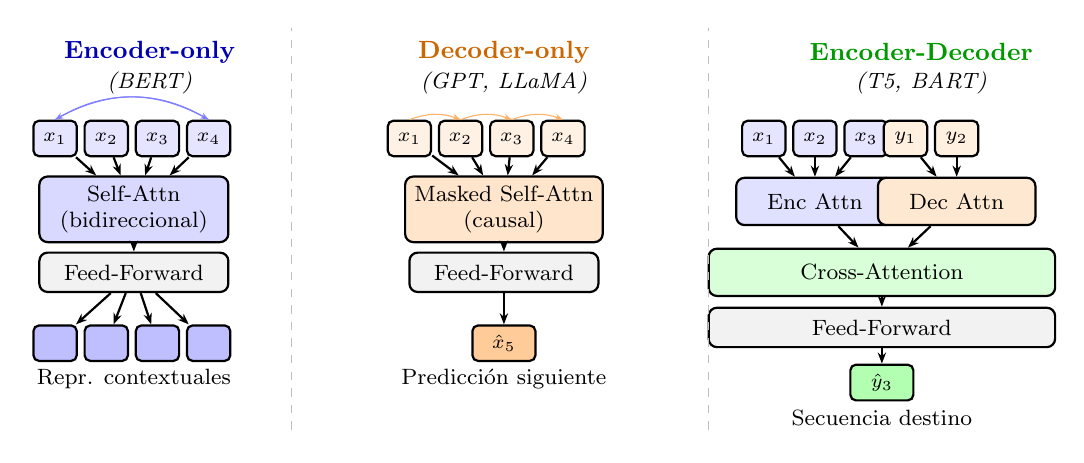
\begin{tikzpicture}[
    tok/.style={draw, rounded corners=2pt, minimum width=0.55cm, minimum height=0.45cm,
                thick, font=\scriptsize},
    attn/.style={draw, rounded corners=3pt, minimum width=2.4cm, minimum height=0.6cm,
                 thick, align=center, font=\footnotesize},
    ff/.style={draw, rounded corners=3pt, minimum width=2.4cm, minimum height=0.5cm,
               thick, align=center, font=\footnotesize, fill=gray!10},
    head/.style={font=\small\bfseries},
    sub/.style={font=\footnotesize\itshape},
    arr/.style={-{Stealth[length=4pt]}, thick},
    endarr/.style={-{Stealth[length=5pt]}, line width=1.2pt}
]

% ============================================================
% ENCODER-ONLY (left column)  x=0
% ============================================================
\node[head, blue!70!black]  at (1.2, 6.8)  {Encoder-only};
\node[sub]                  at (1.2, 6.4)  {(BERT)};

% tokens in
\foreach \i/\w in {0/$x_1$,1/$x_2$,2/$x_3$,3/$x_4$} {
    \node[tok, fill=blue!10] (ei\i) at (\i*0.65, 5.7) {\w};
}
% attn block (bidireccional)
\node[attn, fill=blue!15] (esa) at (1.0, 4.8) {Self-Attn\\(bidireccional)};
\node[ff] (eff) at (1.0, 4.0) {Feed-Forward};
% output representations
\foreach \i in {0,1,2,3} {
    \node[tok, fill=blue!25] (eo\i) at (\i*0.65, 3.1) {};
}
\node[font=\footnotesize] at (1.0, 2.65) {Repr. contextuales};

% arrows
\foreach \i in {0,1,2,3} { \draw[arr] (ei\i) -- (esa); }
\draw[arr] (esa) -- (eff);
\foreach \i in {0,1,2,3} { \draw[arr] (eff) -- (eo\i); }

% bidireccional arrows inside attn
\draw[-{Stealth[length=3pt]}, blue!50, bend left=30] (ei0.north) to (ei3.north);
\draw[-{Stealth[length=3pt]}, blue!50, bend right=30] (ei3.north) to (ei0.north);

% ============================================================
% DECODER-ONLY (center column)  x=4.5
% ============================================================
\node[head, orange!80!black] at (5.7, 6.8)  {Decoder-only};
\node[sub]                   at (5.7, 6.4)  {(GPT, LLaMA)};

\foreach \i/\w in {0/$x_1$,1/$x_2$,2/$x_3$,3/$x_4$} {
    \node[tok, fill=orange!10] (di\i) at (4.5+\i*0.65, 5.7) {\w};
}
\node[attn, fill=orange!20] (dsa) at (5.7, 4.8) {Masked Self-Attn\\(causal)};
\node[ff] (dff) at (5.7, 4.0) {Feed-Forward};

% output: only next token
\node[tok, fill=orange!40, minimum width=0.8cm] (dout) at (5.7, 3.1) {$\hat{x}_5$};
\node[font=\footnotesize] at (5.7, 2.65) {Predicción siguiente};

\foreach \i in {0,1,2,3} { \draw[arr] (di\i) -- (dsa); }
\draw[arr] (dsa) -- (dff);
\draw[arr] (dff) -- (dout);

% causal arrows (only left-to-right)
\foreach \i in {0,1,2} {
    \pgfmathtruncatemacro{\j}{\i+1}
    \draw[-{Stealth[length=3pt]}, orange!60] (di\i.north) to[bend left=20] (di\j.north);
}

% ============================================================
% ENCODER-DECODER (right column)  x=9
% ============================================================
\node[head, green!60!black] at (11.0, 6.8)  {Encoder-Decoder};
\node[sub]                  at (11.0, 6.4)  {(T5, BART)};

% encoder side
\foreach \i/\w in {0/$x_1$,1/$x_2$,2/$x_3$} {
    \node[tok, fill=blue!10] (edi\i) at (9.0+\i*0.65, 5.7) {\w};
}
\node[attn, fill=blue!12, minimum width=2.0cm] (eedsa) at (9.65, 4.9) {Enc Attn};

% decoder side
\foreach \i/\w in {0/$y_1$,1/$y_2$} {
    \node[tok, fill=orange!12] (edo\i) at (10.8+\i*0.65, 5.7) {\w};
}
\node[attn, fill=orange!18, minimum width=2.0cm] (edca) at (11.45, 4.9) {Dec Attn};

% cross attn
\node[attn, fill=green!15, minimum width=4.4cm] (edcross) at (10.5, 4.0) {Cross-Attention};
\node[ff, minimum width=4.4cm] (edff) at (10.5, 3.3) {Feed-Forward};
\node[tok, fill=green!30, minimum width=0.8cm] (edout) at (10.5, 2.6) {$\hat{y}_3$};

\foreach \i in {0,1,2} { \draw[arr] (edi\i) -- (eedsa); }
\foreach \i in {0,1} { \draw[arr] (edo\i) -- (edca); }
\draw[arr] (eedsa) -- (edcross);
\draw[arr] (edca)  -- (edcross);
\draw[arr] (edcross) -- (edff);
\draw[arr] (edff) -- (edout);
\node[font=\footnotesize] at (10.5, 2.15) {Secuencia destino};

% ============================================================
% Dividers
% ============================================================
\draw[dashed, gray!50] (3.0, 2.0) -- (3.0, 7.1);
\draw[dashed, gray!50] (8.3, 2.0) -- (8.3, 7.1);

\end{tikzpicture}
\end{document}
